


\tikzset{every picture/.style={line width=0.75pt}} %set default line width to 0.75pt        

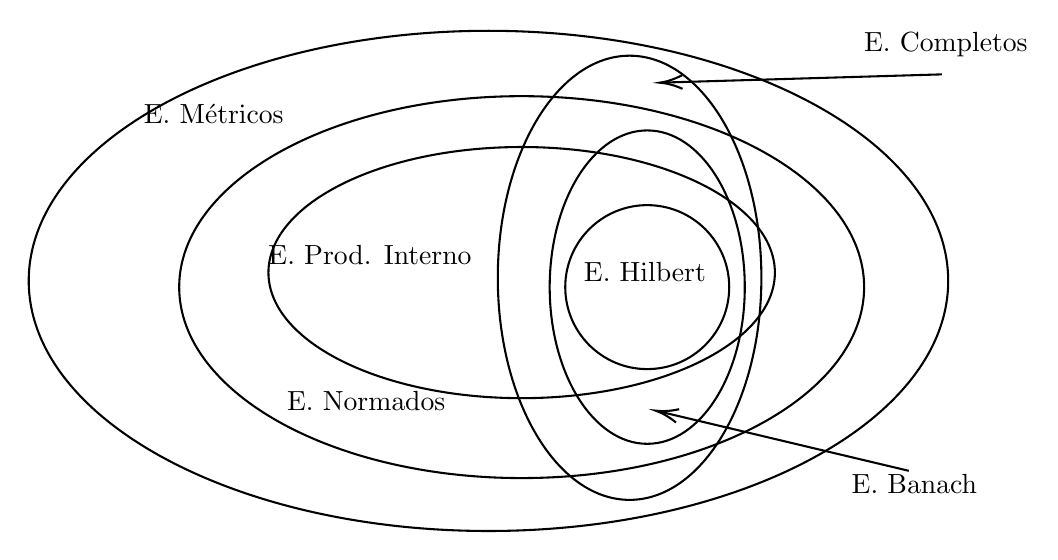
\begin{tikzpicture}[x=0.75pt,y=0.75pt,yscale=-1,xscale=1]
%uncomment if require: \path (0,300); %set diagram left start at 0, and has height of 300

%Shape: Ellipse [id:dp6409032502189613] 
\draw   (92,153.5) .. controls (92,86.95) and (191.17,33) .. (313.5,33) .. controls (435.83,33) and (535,86.95) .. (535,153.5) .. controls (535,220.05) and (435.83,274) .. (313.5,274) .. controls (191.17,274) and (92,220.05) .. (92,153.5) -- cycle ;
%Shape: Ellipse [id:dp11758886757713705] 
\draw   (164.5,156.5) .. controls (164.5,105.69) and (238.37,64.5) .. (329.5,64.5) .. controls (420.63,64.5) and (494.5,105.69) .. (494.5,156.5) .. controls (494.5,207.31) and (420.63,248.5) .. (329.5,248.5) .. controls (238.37,248.5) and (164.5,207.31) .. (164.5,156.5) -- cycle ;
%Shape: Ellipse [id:dp8902248466134244] 
\draw   (207.5,149.5) .. controls (207.5,116.09) and (262.12,89) .. (329.5,89) .. controls (396.88,89) and (451.5,116.09) .. (451.5,149.5) .. controls (451.5,182.91) and (396.88,210) .. (329.5,210) .. controls (262.12,210) and (207.5,182.91) .. (207.5,149.5) -- cycle ;
%Shape: Ellipse [id:dp37785386684302313] 
\draw   (318,152) .. controls (318,92.91) and (346.43,45) .. (381.5,45) .. controls (416.57,45) and (445,92.91) .. (445,152) .. controls (445,211.09) and (416.57,259) .. (381.5,259) .. controls (346.43,259) and (318,211.09) .. (318,152) -- cycle ;
%Shape: Ellipse [id:dp8505854350426449] 
\draw   (343,156.5) .. controls (343,114.8) and (364.04,81) .. (390,81) .. controls (415.96,81) and (437,114.8) .. (437,156.5) .. controls (437,198.2) and (415.96,232) .. (390,232) .. controls (364.04,232) and (343,198.2) .. (343,156.5) -- cycle ;
%Shape: Circle [id:dp9575023540116503] 
\draw   (350.5,156.5) .. controls (350.5,134.68) and (368.18,117) .. (390,117) .. controls (411.82,117) and (429.5,134.68) .. (429.5,156.5) .. controls (429.5,178.32) and (411.82,196) .. (390,196) .. controls (368.18,196) and (350.5,178.32) .. (350.5,156.5) -- cycle ;
%Straight Lines [id:da5993574308661864] 
\draw    (532,54) -- (398,57.94) ;
\draw [shift={(396,58)}, rotate = 358.32] [color={rgb, 255:red, 0; green, 0; blue, 0 }  ][line width=0.75]    (10.93,-3.29) .. controls (6.95,-1.4) and (3.31,-0.3) .. (0,0) .. controls (3.31,0.3) and (6.95,1.4) .. (10.93,3.29)   ;
%Straight Lines [id:da8738920932323038] 
\draw    (516,245) -- (395.95,216.46) ;
\draw [shift={(394,216)}, rotate = 13.37] [color={rgb, 255:red, 0; green, 0; blue, 0 }  ][line width=0.75]    (10.93,-3.29) .. controls (6.95,-1.4) and (3.31,-0.3) .. (0,0) .. controls (3.31,0.3) and (6.95,1.4) .. (10.93,3.29)   ;

% Text Node
\draw (146,67) node [anchor=north west][inner sep=0.75pt]   [align=left] {E. Métricos};
% Text Node
\draw (215,205) node [anchor=north west][inner sep=0.75pt]   [align=left] {E. Normados};
% Text Node
\draw (206,135) node [anchor=north west][inner sep=0.75pt]   [align=left] {E. Prod. Interno};
% Text Node
\draw (358,143) node [anchor=north west][inner sep=0.75pt]   [align=left] {E. Hilbert};
% Text Node
\draw (487,245) node [anchor=north west][inner sep=0.75pt]   [align=left] {E. Banach};
% Text Node
\draw (493,32) node [anchor=north west][inner sep=0.75pt]   [align=left] {E. Completos};


\end{tikzpicture}
